\startcontents[localtoc]
\printcontents[localtoc]{}{0}{\subsection*{Contents}\setcounter{tocdepth}{2}}



\phantomsection
\addcontentsline{toc}{section}{Generate sample data}
\subsubsection*{Generate sample data}



An dependence of amplitude error (Volts, ppm) on signal frequency (Hz) of an ADC was measured and
uncertainties of measurement was estimated. The uncertainty of frequency can be considered as
negligible.

\begin{lstlisting}
%3.7+12.*x+3.*x.^2
f = [10 1e2 1e3 1e4 1e5];
err = [19.700 32.700 69.700 90.700 148.700];
err_unc = [4 10 13 20 33];
\end{lstlisting}


Set independent and dependent variables for \texttt{CCC} algorithm. Lets operate in semi logarithm space
for easy plotting.

\begin{lstlisting}
DI = [];
DI.x.v = log10(f);
DI.x.u = [];
DI.y.v = err;
DI.y.u = err_unc;
\end{lstlisting}


Suppose the ADC has quadratic dependence of the error on the signal frequency.

\begin{lstlisting}
DI.exponents.v = [0 1 2];
\end{lstlisting}


\phantomsection
\addcontentsline{toc}{section}{Call algorithm}
\subsubsection*{Call algorithm}



Use QWTB to apply algorithm \texttt{CCC} to data \texttt{DI}.

\begin{lstlisting}
DO = qwtb('CCC', DI);
\end{lstlisting}
\begin{lstlisting}[language={},xleftmargin=5pt,frame=none]
QWTB: no uncertainty calculation
QWTB: CCC wrapper: model was set by CCC wrapper to a value `Model 2a`.
warning: inline is obsolete; use anonymous functions instead

\end{lstlisting}


\phantomsection
\addcontentsline{toc}{section}{Display results}
\subsubsection*{Display results}



Results is

\begin{lstlisting}
disp(['offset          : ' num2str(DO.coefs.v(1)) ' +- ' num2str(DO.coefs.u(1))])
disp(['linear coeff.   : ' num2str(DO.coefs.v(2)) ' +- ' num2str(DO.coefs.u(2))])
disp(['quadratic coeff.: ' num2str(DO.coefs.v(3)) ' +- ' num2str(DO.coefs.u(3))])
\end{lstlisting}
\begin{lstlisting}[language={},xleftmargin=5pt,frame=none]
offset          : 12.6828 +- 16.9884
linear coeff.   : 1.9434 +- 19.1198
quadratic coeff.: 4.9055 +- 3.9754

\end{lstlisting}


\phantomsection
\addcontentsline{toc}{section}{Interpolate values}
\subsubsection*{Interpolate values}



Interpolate fitted polynom at values \texttt{t}.

\begin{lstlisting}
t = [0:0.1:6];
ty = DO.func.v(t, DO.coefs.v);
\end{lstlisting}


Calculate uncertainties of interpolated values (\texttt{S} is sensitivity matrix, \texttt{CC} is covariance
matrix of coefficients, \texttt{CT} is covariance matrix of interpolated values, \texttt{uty} is uncertainty of
interpolated values).

\begin{lstlisting}
for i = 1:length(t);
        S = t(i).^DI.exponents.v;
        CC = diag(DO.coefs.u,0)*DO.coefs.c*diag(DO.coefs.u,0);
        CT(i)=S*CC*S';
end
uty=CT.^0.5;
\end{lstlisting}


\phantomsection
\addcontentsline{toc}{section}{Plot results}
\subsubsection*{Plot results}

\begin{lstlisting}
hold on
errorbar(DI.x.v, DI.y.v, DI.y.u, 'xb')
errorbar(DI.x.v, DO.yhat.v, DO.yhat.u, 'og')
plot(t, ty, '-r');
plot(t, ty + uty, '-r');
plot(t, ty - uty, '-r');
xlabel('log(f)')
ylabel('error of amplitude')
legend('original data','fitted values','interpolated values', 'uncer. of int. val.','location','southeast')
hold off
\end{lstlisting}
\begin{center}
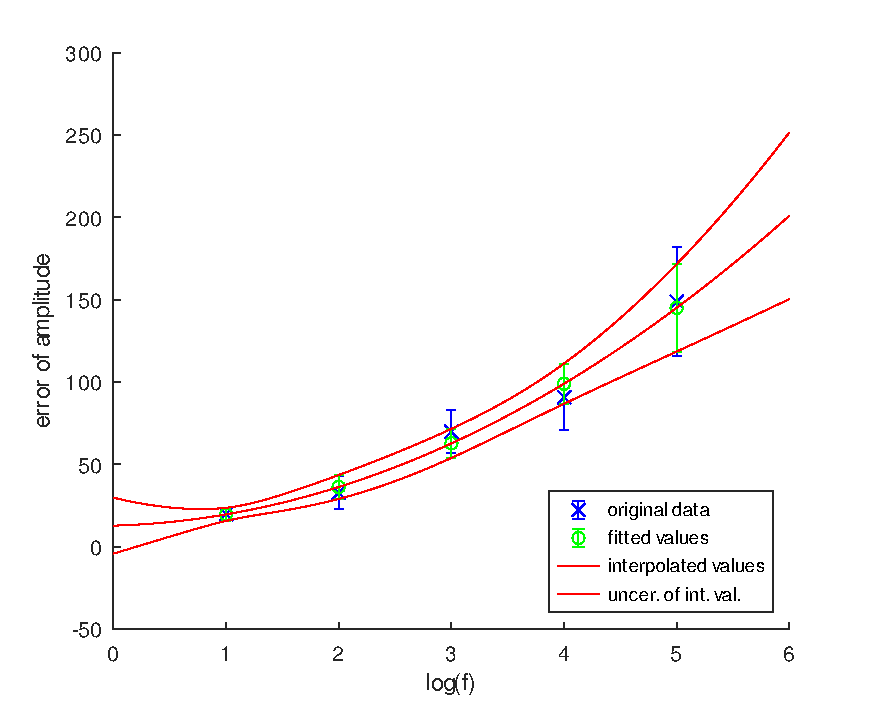
\includegraphics[width=0.7\textwidth]{algs_examples_published/CCC_alg_example-1.pdf}
\end{center}


\stopcontents[localtoc]
